% Created 2020-08-27 Thu 21:05
% Intended LaTeX compiler: pdflatex
\documentclass[11pt]{article}
\usepackage[utf8]{inputenc}
\usepackage[T1]{fontenc}
\usepackage{graphicx}
\usepackage{grffile}
\usepackage{longtable}
\usepackage{wrapfig}
\usepackage{rotating}
\usepackage[normalem]{ulem}
\usepackage{amsmath}
\usepackage{textcomp}
\usepackage{amssymb}
\usepackage{capt-of}
\usepackage{hyperref}
\usepackage{minted}
\IfFileExists{../resources/style.sty}{\usepackage{../resources/style}}{}
\IfFileExists{../resources/referencing.sty}{\usepackage{../resources/referencing}}{}
\addbibresource{../resources/references.bib}
\author{Ryan Greenup}
\date{\today}
\title{Relationship of Model Parameters and Solution Stability in the Power Walk Page Rank Method.}
\hypersetup{
 pdfauthor={Ryan Greenup},
 pdftitle={Relationship of Model Parameters and Solution Stability in the Power Walk Page Rank Method.},
 pdfkeywords={},
 pdfsubject={},
 pdfcreator={Emacs 27.1 (Org mode 9.4)}, 
 pdflang={English}}
\begin{document}

\maketitle
\tableofcontents

\section{Introduction}
\label{sec:org9714071}
Much information is interconnected, consider for example written articles,
research papers, citations, movies, books, personal notes, knowledge bases,
personal releationships etc., this interconnectivity creates a network which can
naturally be visualised as a graph.

Determining the most central vertex of such a graph is useful as it may assist
in research, learning and collaboration. The \emph{PageRank} method, which originally
underpinned \emph{Google}'s search-engine, essentially asserts, that the centre-most
vertex of a graph could be considered the vertex that has the highest
probability of being a destination following a random walk.
\cite{larrypageAnatomyLargescaleHypertextual1998} Although this method is popular,
it does not, however, easily adapt to negatively weighted edges (a negative
weight in this case measuring dissaproval or an aversion to follow that link as
opposed to endorsement). This limitation is increasingly relevant given
recent developments in the area of \emph{Sentiment Analysis}.
\cite{parkPowerWalkProceedings2013}

The \emph{Power Walk} Method is similar to the \emph{Random Surfer} model but takes a
different approach in order to accommodate the potential for an edge to have any
arbitrary real weight. \cite{parkPowerWalkProceedings2013}

This research project will be an investigation into the relationship between
model parameters and the solution stability of the \emph{Power Walk} method.

\subsection{Motivation}
\label{sec:org7f944a8}

Taking advantages of inter-related ideas allows for exploratory research which
can promote both a deeper and broader understading of a topic, an example of
this is the concept of a \emph{pathfinder}, which is a list of central sources for a
topic that can help in early stages of literature searches,
\cite{harbesonTeachingReferenceBibliography1972}
examples of such Pathfinders include:

\begin{itemize}
\item Institution examples:
\begin{itemize}
\item \href{https://libraries.mit.edu/experts/}{\emph{M.I.T.}} \cite{mitResearchGuidesExpert}
\item \href{https://guides.library.harvard.edu/}{\emph{Harvard}} \cite{harvarduniversityResearchGuides}
\item \href{https://www.lib.berkeley.edu/libraries/business-library}{Berkley University} \cite{berkleyuniversityBusinessLibraryUC}
\item \href{https://www.loc.gov/rr/scitech/tracer-bullets/}{\emph{Library of Congress}} \cite{ScienceTracerBullets}
\begin{itemize}
\item The Library of Congress refers to a \emph{PathFinder} as a \emph{Tracer Bullet}, which is both a very descriptive and very American name.
\end{itemize}
\end{itemize}
\item Wiki Examples:
\begin{itemize}
\item \href{http://mathonline.wikidot.com/}{Math Online}  \cite{Mathonline}
\item \href{https://brilliant.org/wiki/best/}{\emph{Brilliant} Wiki} \cite{Top100Wiki}
\item \href{https://www.mediawiki.org/wiki/Help:Categories}{Category Pages within MediaWiki Sites} \cite{HelpCategoriesMediaWiki}
\begin{itemize}
\item For example the \href{https://en.wikipedia.org/wiki/Category:Mathematics}{\emph{Wikipedia} Mathematics Category Page} \cite{CategoryMathematics2019}
\end{itemize}
\end{itemize}
\end{itemize}

Using \emph{Wikipedia} for example can make for a very effective subject guide by
following the various hyperlinks across wikipedia and leveraging \href{https://www.mediawiki.org/wiki/Help:Categories}{Category Pages}
\cite{HelpCategoriesMediaWiki} in order to map out a topic while referring to
references as necessary. Such a strategy is even recommended by some \href{https://mville.libguides.com/c.php?g=370066\&p=2500344}{Library
Study Guides} \cite{moskowitzLibraryGuidesWikipedia}, and has even been implemented
in recommendation systems to overcome limitations imposed by a lack of data
\cite{loizouUsingWikipediaAlleviate2010a} (see section \ref{wiki-networks}).

Similarly the \href{https://en.wikipedia.org/wiki/Collective\_Knowledge\_(software)}{\emph{Zettelkasten} method} of note taking involves, in essence, a
collection of small interlinked notes \cite{OverviewZettelkastenMethod}, much like
a wiki, within the last two decades this method has peaked in popularity
\cite{GoogleBooksNgram}, despite being a method dating back to atleast the 18th
Century. \cite{haarkoetterAllesWesentlicheFindet} This is likely driven, atleast
in part, by the development of the internet, \emph{HTML} and the increasing breadth
and depth of human knowledge.

A comprehensive review of the pathfinder approach, however, reveals that many
such subject guides are often not consistent with the needs of those engaging in
research. \cite{vilenoPaperElectronicEvolution2007} This issue is somewhat
analogous to the work of Larry Page and Sergey Brin when developing
\emph{Google} in that the centrality of an article of information corresponds very
greatly to it's relevance. \cite{larrypageAnatomyLargescaleHypertextual1998}

This issue of relevance in information retrieval can be addressed by using an
algorithm to identify what is most central to a topic, ideally the \emph{Power Walk}
method will prove to be an effective tool to achieve this.

\section{Background and Rationale}
\label{sec:org8173e6b}
Given some graph \(G(V,E)\) with \(\mid V \mid = n\), a corresponding adjacency
matrix \(\mathbf{A}\) describes the number of edges between vertex \(i\) and \(j\),
such that \(\mathbf{A}_{i, j}\) represents the number of edges between the
vertices.

With respect to a directed graph the element \(\mathbf{A}_{i, j}\) may either denote the edge:

\begin{itemize}
\item \(i \rightarrow j\)
\begin{itemize}
\item One such example of this implementation being the \texttt{igraph} library \cite{gaborcsardiIgraphManualPages2019}
\end{itemize}
\item \(j \rightarrow i\) \cite[\textsection 2.3]{nicholsonLinearAlgebraApplications2009}, OR
\end{itemize}

While both definitions appear in the literature, the latter definition is more
common/convenient when working with \emph{probability transition matrices} and will
hence be adopted here.
\subsection{Stationary Distribution}
\label{stationary-distribution}
Given this adjacency matrix \(\mathbf{A}\), a \emph{probability transition matrix}
\(\mathbf{T}\) can be produced by scaling each column to 1, such that each element
\(\mathrm{T}_{i, j}\) would represent the probability of leaving \(j\) and
travelling to \(i\) during a random walk (as opposed to the number of edges as was
the case with \(\mathbf{A}\)), this can
be acheived with matrix multiplication as illustrated in
\eqref{eq:mat-mult-colsum}:

\begin{align}
\mathbf{T} = \mathbf{A} \enspace \mathrm{diag}\left( \mathtt{colsums}\left(
\mathbf{A} \right) \right) \label{eq:mat-mult-colsum} \end{align}

The state distribution \(\vec{p}_{k}\) describes the frequency (scaled to 1) of
visiting each vertex during a random walk for the \(k^{\textrm{th}}\) step of the
walk, given this, the stationary distribution \(\vec{p}\) is given by
\eqref{eq:stationary-distribution}:


\begin{align}
\vec{p_{i}} &= \mathbf{T} p_{i-1} \nonumber \\ \lim_{n \to \infty} \left[
\vec{p_{i}} \right] &= \lim_{n \to \infty} \left[ \mathbf{T} \vec{p_{i-1}}
\right] \nonumber \\ \implies \vec{p} &= \mathbf{T} \vec{p}
\label{eq:stationary-distribution} \end{align}

If \(G(V, E)\) is an ergodic graph (i.e. all vertices may be reached from any
initial vertex), this can be solved by iteration by setting some threshold
\((\eta)\) for convergence (which will be referred to as the \emph{Power Method}) or by
solving the eigenvalue problem for \(\lambda=1\) as shown in \eqref{eq:eigen-one}:

\begin{align}
\lambda \vec{p} &= \mathbf{T} \vec{p} \nonumber \\ \lambda = 1 \implies \vec{p}
&= \mathbf{T} \vec{p} \label{eq:eigen-one} \end{align}

\subsection{Random Surfer}
\label{sec:orgda80ae1}
If however a graph is non-ergodic, this random walk will not traverse every
vertex, to overcome this, the \emph{Random Surfer} model can be implemented
\cite{larrypageAnatomyLargescaleHypertextual1998}. This method involves,
essentially, introducing into the \emph{probability transition matrix}
\((\mathbf{T})\), some probability \((\frac{1-\alpha}{n})\) of traversing to a
disconnected vertex \((V)\), this is shown in \eqref{eq:random-surfer}:

\begin{align}
\mathbf{T}_{\textrm{RS}} = \mathbf{S} = \alpha \mathbf{T} + (1-\alpha) \mathbf{B}
\label{eq:random-surfer} \end{align}

where:

\begin{itemize}
\item \(\mathbf{B}\) is matrix of size \(n \times n\) such that \(\mathbf{B}_{i, j} = \frac{1}{n}, \enspace \forall i,j \in \left[1, n\right]\cap \mathbb{N}\)
\item In the literature \(\alpha\) is often referred to as a damping factor see
\cite{berkhoutRankingNodesGeneral2018a,brinkmeierPageRankRevisited2006a,fuDampingFactorGoogle2006,kamvarAdaptiveMethodsComputation2004b,bianchiniPageRank2005}
or a smoothing constant \cite{koppelMeasuringDirectIndirect2014} .
\end{itemize}

\subsection{Power Walk}
\label{sec:org217af8c}
The random surfer model \eqref{eq:random-surfer}, however, assumes that all edges are an edorsement of
the target, i.e. they are weighted positively, the power walk method
\cite{parkPowerWalkProceedings2013}, shown in \eqref{eqref:eq:power-walk-method}, takes a
different approach to create a \emph{transition probability matrix} \((\mathbf{W})\) and is compatible
with a negatively weighted edges:

\begin{align}
\mathbf{W}_{i, j} &= \frac{\beta^{\mathbf{A'}{i, j}}}{\sum^{n}_{j = 1} \left[
\beta^{a_{i, j}} \right]} \label{eqref:eq:power-walk-method} \end{align}


where:

\begin{description}
\item[{\(\mathbf{A'}\)}] is a weighted adjacency matrix such that \(\mathbf{A}_{i, j} \in \mathbb{R}\)
\item[{\(x\)}] is the probability of travelling to a vertex for which there is no connection.
\begin{itemize}
\item Similarly to \eqref{eq:random-surfer} , \(x = \frac{1-\alpha}{n}\)
\end{itemize}
\item[{\(\mathbf{\beta}\)}] is the ratio of probability between following an edge and
making a jump to a vertex for which there is no path
\begin{itemize}
\item i.e. \(\beta x\) is the probability of following a path with a weight of 1.
\end{itemize}
\end{description}

\subsection{Solving the stationary distribution}
\label{iterative-power-method}
Solving the EigenValue problem for a large matrix can be very resource
intensive, for example \emph{Wikipedia} currently has over 6, 000, 000 pages
\cite{WikipediaSizeWikipedia2020} which would correspond to an adjacency matrix
with over \(10^{12}\) entries, yet even a relatively fast compiled language like
\emph{Julia} can struggle to solve the eigen vectors for a matrix of size
\((10^{4})^{2}\) as shown in listing \ref{eigen-julia}.

The power method, first mentioned in section \ref{stationary-distribution}, is a
better suited approach, with respect to performance, because:

\begin{enumerate}
\item The method is only looking for one solution
\item The accuracy of the solution (measured by  \(\exists\eta\in \mathbb{R}\)) can be tuned to improve performance.
\end{enumerate}



\begin{listing}[htbp]
\begin{minted}[]{julia}
using LinearAlgebra
using TimerOutputs

function time_eigenvec(n)
    T = [ x-n+n*y for x in rand(n), y in rand(n) ]
    t = @elapsed eigvecs(T) return t end

time_eigenvec(10^2)
time_eigenvec(10^3)
# time_eigenvec(10^4) # times out


## : time_eigenvec (generic function with 1 method)
## : 0.072302487
## : 0.814937083
\end{minted}
\caption{\label{eigen-julia}Time to Solve Eigen Value for matrix of size \(n\)}
\end{listing}

\section{Proposed Research}
\label{sec:orgaf690e4}
Consider the ordered set of EigenVectors \eqref{eq:eigen-set} of a positive
transition probability matrix such as \(\mathbf{S}\) \eqref{eq:random-surfer} or
\(\mathbf{T}\) \eqref{eq:stationary-distribution}:

\begin{align}
\{ \lambda_{k} \mid \enspace  \lambda_{k} < \lambda_{k-1}, \enspace k\in \mathbb{Z}^{+} \leq n \} \label{eq:eigen-set}
\end{align}

\subsection{Dominant EigenVector}
\label{sec:org5e37979}
It has been shown that \(\lambda_{k} \leq 1, \enspace \forall k \leq n\) and that the dominant\footnote{Dominant in this case refers to the the largest \(\mid \lambda_{k} \mid\)} \(\lambda\) can be computed by the \emph{power method}. \cite{farahatAuthorityRankingsHITS2006}


\subsection{Stability and Convergence}
\label{stability-convergence}
It has also been shown that the stationary distribution \(\vec{p}\) (see
\eqref{eq:stationary-distribution} ) can be reached in a limited number of steps
(\(\approx 50\)) for graphs on the order of a million vertices
\cite[p. 123]{bianchiniPageRank2005}, under the assumption that the
smoothing constant \(\alpha \in \left[0, 1\right]\) is not too close to 1 (in
which case convergence can become quite slow)
\cite{tanNewExtrapolationMethod2017a}

How quickly the \emph{Power Method} converges generally depends on the magnitude of \(\mid \lambda_{2} \mid\) \cite{bryan250000002006}
and with respect to the random surfer model \eqref{eq:random-surfer}, It has been shown
that: \cite{kamvarAdaptiveMethodsComputation2004b}

\begin{itemize}
\item \(\mid \lambda_{2} \mid \leq \alpha\), and
\item if the corresponding graph contains two or more irreducible closed subgraphs
then \(\mid \lambda_{2} \mid = \alpha\)
\end{itemize}

This is demonstrated in listing \ref{random-surf-r} and figure \ref{two-sub-graph}.

It has also been shown that an \(\alpha\) value near 1 will imply an unstable
stationary distribution \cite{ngStableAlgorithmsLink2001} that converges slowly
\cite{tanNewExtrapolationMethod2017a}, this is because \(\lambda_{2}\) is bound above by
\(\alpha\) and a small change to the corresponding graph could lead to
\(\lambda_{1} \leftrightarrow \lambda_{2}\) and hence different eigenvectors will
correspond to the solution as shown in \eqref{eq:eigen-one} .

It is not clear how similar properties are exhibited with respect to the \emph{Power Walk} method. \cite{parkPowerWalkRevisiting2013}

\subsection{Choosing \(\alpha\)}
\label{choosing-alpha}
Although section \ref{stability-convergence} might suggest that smaller values of
\(\alpha\) may be more ideal, it is worth recalling that as \(\alpha\) is reduced
the probability of a random walk visiting any other vertex will become more and
more uniform because \(\frac{1-\alpha}{n} \rightarrow \frac{1}{n}\) as \(\alpha
\rightarrow 0\). \cite{parkPowerWalkRevisiting2013}

The value used originally by Page and Brin was \(\alpha = 0.85\) See
\cite[p. 109]{larrypageAnatomyLargescaleHypertextual1998} and this appears to have been
widely adopted, see
\cite{kamvarAdaptiveMethodsComputation2004b,boldiPageRankFunctionDamping2005}.
Research suggests, however, that modifying the value may be useful in detecting
spam.
\cite{zhangMakingEigenvectorBasedReputation2004,boldiPageRankFunctionDamping2005}


\begin{listing}[htbp]
\begin{minted}[]{r}
library(igraph)
library(tidyverse)

g1 <- igraph::graph.formula(1++2, 1+-8, 1+-5, 2+-5, 2+-7, 2+-8, 2+-6, 2+-9, 3++4, 3+-5, 3+-6, 3+-9, 3+-10, 4+-9, 4+-10, 4+-5, 5+-8, 6+-8, 7+-8)

A <- igraph::get.adjacency(g1, names = TRUE, sparse = FALSE) %>%
  as.matrix()

## Adjust the Order
A <- A[order(as.integer(row.names(A))), order(as.integer(colnames(A)))]

adj_to_probTrans <- function(adjMat) {
  t(adjMat) %*% diag(1/colSums(t(adjMat)))
}

B <- matrix(rep(1/nrow(T), length.out = nrow(T)**2), nrow = nrow(T))
ɑ <- 0.123456789

S <- ɑ*T+(1-ɑ)*B


eigen(S, symmetric = FALSE)$values


## [1]  1.000000e+00 -1.234568e-01  1.234568e-01 -1.234568e-01  2.231012e-10
## [6] -2.231012e-10 -8.488298e-18  3.570154e-18 -1.450336e-20  9.629650e-35
\end{minted}
\caption{\label{random-surf-r}Implementing the random surfer model for the graph shown in figure }
\end{listing}

\begin{figure}[htbp]
\centering
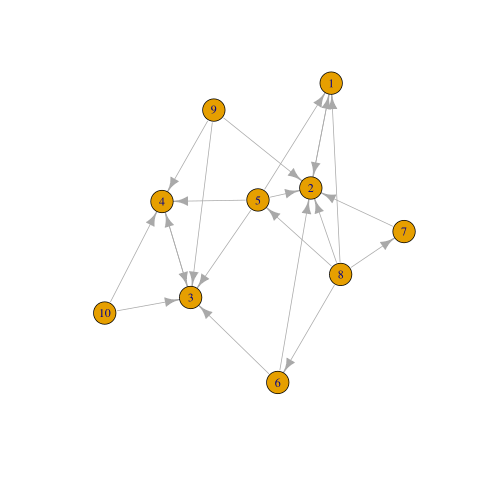
\includegraphics[width=.9\linewidth]{two-sub-graph-fig2.png}
\caption{\label{two-sub-graph}Graph with two closed irreducible subgraphs}
\end{figure}

\subsection{Research Question}
\label{research-question}
It is not clear how \(\lambda_{2}\) behaves with respect to the \emph{Power Walk} method, \eqref{eqref:eq:power-walk-method} although it has been shown that under specific circumstances the value of \(\mid \lambda_{2}\mid\) can be predicted from the method parameters and properties of the graph. \cite[\textsection 3.4]{parkPowerWalkProceedings2013}

This research will involve investigating the relationship between the second eigenvalue of the \emph{Power Walk} transition matrix and the features of a graph corresponding to some type of network (e.g. a social network, webpages, wiki, etc.)

In particular, open questions are whether or not the value of the second eigenvalue can:

\begin{itemize}
\item be predicted from the parameters of the model and/or features of the graph
\begin{itemize}
\item e.g. some function of \(\alpha\) / \(\beta\)
\end{itemize}
\item indicate the stability of the stationary distribution of a graph
\item indicate how quickly the \emph{Power Method} will converge to a solution
\end{itemize}

\section{Literature Review}
\label{summary-lit-review}
The proposed research (see section \ref{research-question}) relates broadly to the \emph{PageRank} method, Random-Surfer model, sentiment
analysis and graph centrality, for which material is quite abundant, although much
of the literature is concerned with either:

\begin{enumerate}
\item The original \emph{PageRank} method developed by Page and Brin \cite{larrypageAnatomyLargescaleHypertextual1998}
\item Modifying the \emph{PageRank} method to improve upon:
\begin{itemize}
\item Precision and accuracy see \cite{ngStableAlgorithmsLink2001,berkhoutRankingNodesGeneral2018a,nemaConsensusbasedRankingWikipedia2017a,fuDampingFactorGoogle2006}
\item Performance with respect to:
\begin{itemize}
\item Rate of convergence in terms of iterations and time, see \cite{tanNewExtrapolationMethod2017a,langvilleReorderingPageRankProblem2006}
\item Stability of any given solution, see \cite{ngStableAlgorithmsLink2001}
\end{itemize}
\end{itemize}
\end{enumerate}

Although neither of these points are a direct analogue for the proposed
research, which relates in itself to an alternative \emph{PageRank} algorithm, much of
the work will be very similar in approach and hopefully offer much insight upon
closer inspection.

\subsection{Building on Literature Referred to in Primary Resource}
\label{sec:org6b6fa0a}
This research is focused primarily on the \emph{Power Walk} method
proposed by Park and Simoff in a 2013 conference paper,
\cite{parkPowerWalkProceedings2013} this paper contained some discussion of
relevant research.
\subsubsection{Stability and Convergence}
\label{stability-convergence-lit-review}
Haveliwala and Kamvar \cite{haveliwalaSecondEigenvalueGoogle2003} proved that
\(\lambda_{2}\) (see \eqref{eq:eigen-set}) is bounded above by the smoothing
constant \(\alpha\) and in the case that the corresponding graph has more than 1
closed subgraph is equal to \(\alpha\). This is an important revelation because it
has been shown that the further the second eigenvalue is from 1, the more
resistant the stationary distriubtion of the \emph{PageRank} is to perturbations in the
corresponding graph, \cite{ngStableAlgorithmsLink2001} and the faster the \emph{PageRank}
will converge \cite{bryan250000002006}.

It has been shown that the \emph{power method} (see section \ref{iterative-power-method})
will always converge \(\forall \alpha <1\) \cite{bianchiniPageRank2005} and that an
\(\alpha\) closer to the value of 1 does not necessarily correspond to a more
meaningful ranking, \cite{boldiPageRankFunctionDamping2005} hence, given the upper
bound of \(\lambda_{2} \leq \alpha\), the value of \(\alpha\) can be tuned away from
1 in order to improve the convergence and stability of the \emph{PageRank} (however a
value of \(\alpha\) that is too small will indeed be meaningless as discussed in
section \ref{choosing-alpha}). \cite{parkPowerWalkRevisiting2013}

This works provides a framework for considering the method parameters and
\(\lambda_{2}\) with respect to the convergence and stability of the \emph{Power Walk}
method.

\subsubsection{Building on the Random Surfer}
\label{wiki-networks}
Related work referred to in the paper has involved using community ratings of
web pages to improve upon the \emph{PageRank} method
\cite{parkMiningWebMultiresolution2007}, similar work has also been undertaken
more recently that found replacing the background probability \(\frac{1}{n}\) with a combination of usage statistics and content quality
scores can significantly improve the precision and accuracy of the page rank
method. \cite{nemaConsensusbasedRankingWikipedia2017a}

Such a strategy is however limited to websites that make usage statistics
public, such as wikis.

An extension to this research could involve an investigation into the precision
of the \emph{Power Walk} method in conjuction with usage statistics compared with the
\emph{Power Walk} method.


There is literature suggesting that the network structure of wiki articles can
be an important feature in the emergence of quality
\cite{ingawaleNetworkAnalysisUser2013a}, related work also shows that \emph{Wikipedia}
can be used to improve performance of recommender systems when there is limited
data \cite{loizouUsingWikipediaAlleviate2010a} and it would be very interesting to
see how the \emph{Power Walk} method would perform compared to the \emph{PageRank} method
in those situations.

\subsection{Page Rank}
\label{sec:org1725de2}
\subsubsection{Building on the \emph{PageRank} Method}
\label{sec:orgf274bb5}
The \emph{PageRank} method is a relatively versatile approach\footnote{The approach has even been used in conjuction with linear regression to map gene expresseions, see \cite{zhangModifiedPageRankAlgorithm2018}} that is
relatively robust to manipulation compared with other methods for dealing with
information retrieval, \cite{langvilleSurveyEigenvectorMethods2005} perhaps for
this reason there is much literature on modifying the \emph{PageRank} method to
improve upon it as discussed generally in section \ref{summary-lit-review}.

Choosing a smoothing constant, however, is a somewhat difficult task because it can have an
impact on the behaviour of the model (see \cite{fuDampingFactorGoogle2006} and  section
\ref{stability-convergence-lit-review}) but also because without empirical guidance
it can feel somewhat arbitrary, there is an approach in the literature that
involves using input/output ratios to determine an appropriate value
\cite{fuDampingFactorGoogle2006} and another that seeks to use structural network
dynamics to provide a score distribution and obviate the need for a smoothing
constant entirely. \cite{berkhoutRankingNodesGeneral2018a}

It is not entirely clear if this approach will offer much to this method but a
more careful inspection may reveal helpful perspectives.
\subsubsection{Stability and Convergence}
\label{sec:org058644a}
Improving the rate of convergence of the \emph{PowerRank} is obviously desirable and
there has been considerable mathematical resarch to develop better algorithms.

As previously mentioned in \ref{stability-convergence}, the stability and convergence
of the \emph{Power Rank} method is poor when the smoothing constant \(\alpha\) is close
to 1, a 2016 paper published in the \emph{Journal of Computational and Applied
Mathematics} \cite{tanNewExtrapolationMethod2017a} found that the trace of a
matrix can be used to produce a considerably more efficient approach to solve
the \emph{PageRank} for values of \(\alpha\) near 1. It is not clear how relevant this
is given that \(\alpha\) values near 1 offer no improvement in precision
\cite{boldiPageRankFunctionDamping2005} and that the solution is unstable
\cite{ngStableAlgorithmsLink2001} (see sections \ref{choosing-alpha} and
\ref{stability-convergence}), but, it is yet to be shown if these characteristics
necessarily apply to the \emph{Power Walk} method and such an approach may prove to
be insighful nonetheless.

Another approach involves involves reordering the problem and taking advantage
of the fact that the transition probability matrix is sparse \footnote{if an adjacency matrix and/or corresponding probability transition matrix were not sparse each vertex would be like an index, which is unlikely} in order
to produce a new algorithm which cannot perform worse than the \emph{power method}
but has been shown to improve the rate of convergence in certain cases.
\cite{langvilleReorderingPageRankProblem2006}.

\subsubsection{Insightful Miscellaneous Work}
\label{sec:org9c37836}
\paragraph{\emph{PageRank} as a Power Series}
\label{power-series}
Research has shown that the \emph{PageRank} Method can be expressed as a power series
and an algorithm for calculating the page rank derived,
\cite{brinkmeierPageRankRevisited2006a} the solution corresponds to the \emph{power
method} but a slightly faster algorithm is also presented. Seperate work has
been undertaken to similarly express the PageRank in terms of a \emph{McLaurin
Series}, finding that each partial sum of the series corresponds to an iteration
of the \emph{power method}. \cite{boldiPageRankFunctionDamping2005} This work is
extremely relevant to the \emph{Power Walk} method because the exponent in that
method (see \eqref{eqref:eq:power-walk-method}) suggests that an generating
function such as \(f(x) = \sum^n_{i=0} \left[ x^n \frac{a}{n!} \right]\) may be
able to show a more direct relationship between the \emph{PowerRank} and \emph{Power Walk}
approaches.

\paragraph{Modelling}
\label{sec:org6f6048d}
The \emph{PageRank} method has been leveraged as a value to assist in building
artificial networks in order to model real-world networks, such networks have
been shown to have upper and lower bounds on there diamaters.
\cite{mehrabianItSmallWorld2016} This is a very interesting area of research and
it would be interesting to see whether or not the use of the \emph{Power Walk} method
in such an approach produces graphs that are more consistent with social
networks.

\paragraph{Pure Mathematics}
\label{sec:org32c0521}
One very interesting piece of work in the literature was an application
of the \emph{PageRank} method to a graph of integers
with edges based on divisors, as shown in figure \ref{pure-math-graph} and listing \ref{pure-math-adj}. \cite{frahmPageRankIntegers2012}

This is well outside the scope of this research, but if the precision of the
power walk method is found to be reasonably good, it would make for a very
interesting exercise to measure it's performance at predicting integers and
attempting to find relationships between the two.

Another paper outside the scope of this paper is work by Ding \& Li concerned
with extending the \emph{PageRank} method to \emph{multi-plex} graphs\footnote{Multi-plex, in this case, refers to edges between vertices accross
different dimensions, for example a link from a webpage to a food outlet could
be made by way of a hyperlink, a phone number and a street address, this would
be 3 different types of edges between two vertecies and so would be multi-plex.}, although
very interesting and quite practical, such research is beyond the scope of this work.

\begin{listing}[htbp]
\begin{minted}[]{r}
library(igraph)
library(tidyverse)
g1 <- igraph::graph.formula(30-15, 30-5, 30-6, 30-3, 30-2, 29, 28-7, 28-4, 28-2,
27, 26-13, 26-2, 25-5, 24-8, 24-4, 24-2, 24-6, 24-3, 23, 22-11, 22-2, 21-3,
21-7, 20-5, 19, 18-2, 18-3, 18-9, 17, 16-4, 16-2, 16-8, 15-3, 15-5, 14-7, 14-2,
13, 12-4, 12-3, 12-2, 11, 10-5, 10-2, 9-3, 8-2, 8-4, 7, 6-3, 6-2, 5, 4-2, 3, 2)

plot(g1)
\end{minted}
\caption{\label{pure-math-adj}\emph{PageRank} Probability Transition Matrix of network based on divisibility of \(\mathbb{Z}^+ \leq 30\)}
\end{listing}

\begin{figure}[htbp]
\centering
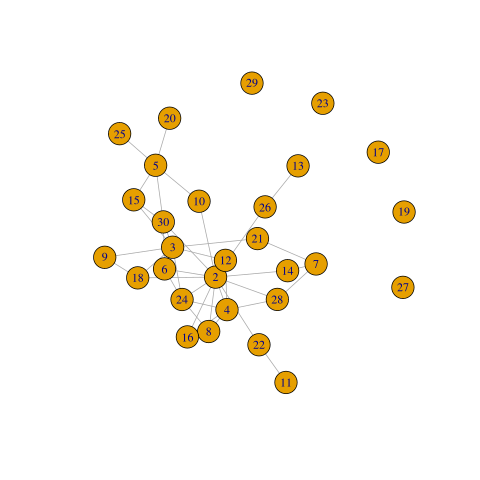
\includegraphics[width=.9\linewidth]{pure-math-adj-graph.png}
\caption{\label{pure-math-graph}Graph of \(\mathbb{Z}^+ \leq 30\) with edges based on divisors}
\end{figure}


\subsection{Search Engine Optimisation}
\label{sec:org6a5f93a}
There is a considerable amount of work in the literature concerning the
relationship between the \emph{PageRank} method and Search Engine optimisation, such
as:

\begin{itemize}
\item Using decision trees with machine learning to inductively model search engines \cite{pringleWhatTallPoppy1998}
\item Methods to solve the optimisation problem involved in centring a vertex by
creating a limited number of edges
\cite{kamvarAdaptiveMethodsComputation2004b,dekerchoveMaximizingPageRankOutlinks2008}
\begin{itemize}
\item Consider a website trying to maximise exposure for example
\item Related papers consider also keyword frequency, see for example \cite{zhangImpactWebpageContent2005}
\end{itemize}
\end{itemize}

Such literature however is suited to an ex post facto study and is hence not
terribly relevant to the proposed research.
\end{document}
